\chapter{Contexto}

Esse projeto tem natureza multidisciplinar, buscando harmonizar a bioquímica do
processo de produção de cervejas com sistemas de controle e automação e
geração e análise de dados estudados na Engenharia Elétrica. Em sua primeira
parte, será estudado o funcionamento das leveduras e como o ambiente age sobre
seu processo metabólico, enquanto na outra parte, são estudados sensores,
atuadores e arquitetura de Internet das Coisas para captação, processamento e
disponibilização de informações referente a ação dos microrganismos.

\section{História da Cerveja}



\section{Fabricação de Cervejas}

O processo de fabricação de cervejas é conhecido pela 
humanidade há milhares de anos, tendo seu primeiro registro histórico em 2800 a.C.
na região da Mesopotâmia. Ao longo dos anos, foi amplamente praticado e estudado
por diversos povos, sendo refinado à medida que um maior compreendimento sobre
o processo foi obtido. Ainda que existam variações dependentes de ingredientes, a
produção de cervejas é dividida por Kunze (\citeonline{Kunze}) nas seguintes etapas: 

\begin{enumerate}
    \item Maltagem dos grãos: comumente cevada, que consiste na produção de
enzimas como a amilase, a partir da germinação controlada e parcial dos
grãos, que passam a ser chamados de malte;
    \item Moagem do malte: expondo as enzimas e componentes internos. É desejável
que parte da casca seja mantida intacta para auxiliar na filtragem após a
mostura;
    \item Mostura: o malte moído é misturado em água, e aquecida em temperaturas
que estimulem a ação das enzimas obtidas na maltagem. As enzimas
realizam a quebra de moléculas insolúveis de amido em moléculas menores
de açúcares, que são dissolvidas, formando o mosto;
    \item Lautering: separação do mosto do resto do malte que não foi dissolvido. As
cascas dos grãos auxiliam essa etapa formando um filtro natural;
    \item Fervura: o mosto é fervido por pelo menos uma hora, a ação enzimática é
interrompida, a solução é esterilizada e lúpulos são adicionados em diferentes
momentos da fervura, fornecendo extratos que conferem amargor, sabor e
aroma à cerveja;
    \item Fermentação: leveduras são adicionadas ao mosto após seu resfriamento e
aeração. Os açúcares são consumidos pelo metabolismo das leveduras,
gerando etanol e dióxido de carbono;
    \item Maturação: após o consumo dos açúcares, as leveduras passam a reabsorver
subprodutos da fermentação, melhorando a qualidade da bebida. As
leveduras então floculam e decantam;
    \item Envase: transferência para o recipiente final. Nessa etapa, também é
realizada a carbonatação da bebida, geralmente por injeção de gás carbônico
ou por meio de uma segunda fermentação, aproveitando-se as leveduras.
Industrialmente, é comum a filtragem pré-envase, e a pasteurização pós-
envase.
\end{enumerate}

\subsection{Fermentação e Maturação}

Segundo descrito por White e Zainasheff (\citeonline{YeastWhite}), as primeiras produções de
cervejas datam de milhares de anos atrás, sendo que na maior parte da história a
fermentação de bebidas foi tida como um fenômeno divino, sem o conhecimento dos
organismos microscópicos que a realiza. Estes só puderam ser observados em 1680
com o desenvolvimento e auxílio de microscópios. Ainda assim, apenas em 1789 a
equação química da transformação de açúcares em álcool, dentre eles o etanol, e
dióxido de carbono ($\mathrm{CO_2}$) foi descrita por Lavoisier, e na segunda metade do século
XIX, com as descobertas de Pasteur, passaram a ser melhor entendidas, com o
surgimento da bioquímica como uma área de estudo própria. 


Apesar da falta de conhecimento durante tantos anos, a fermentação é o processo
que possui um dos maiores impactos no sabor, aroma, aparência e textura do
produto. Sendo assim, o controle dessa etapa é essencial para garantir a
qualidade final.  


A fermentação, na produção de cervejas, é um processo metabólico realizado pelas
leveduras adicionadas ao mosto com a finalidade principal de converter os açúcares
extraídos dos grãos maltados no processo de brassagem em etanol. As leveduras,
fungos unicelulares, realizam a fermentação como uma forma de
respiração anaeróbia para obterem energia em meios desprovidos de oxigênio ou
com grande excesso de açúcares disponíveis. Além da geração de etanol e gás
carbônico, há diversos subprodutos, como ésteres, álcoois superiores e compostos
sulfúricos que caracterizam o produto e definem sua qualidade final. 


O processo de fermentação pode ser dividido em 3 fases:  
\begin{enumerate}
    \item Fase de retardamento, durante as primeiras quatro a 15 horas após a adição
da levedura no mosto, caracterizada pela climatização das células ao
ambiente e preparação para a próxima fase;
    \item Fase de crescimento exponencial, que dura entre quatro horas e quatro dias,
quando ocorre o consumo dos açúcares e replicação logarítmica das células
de leveduras;
    \item Fase estacionária, em que o crescimento diminui e alguns compostos são
absorvidos pelas células, maturando o produto durante três a dez dias.
\end{enumerate}


Para a obtenção de resultados consistentes em testes e na produção de cervejas, é
essencial que a fermentação seja monitorada e controlada de forma que ocorra em
condições ideais. As principais variáveis monitoradas no processo, em ordem de
importância são: a temperatura, que impacta diretamente no grau de atividade
celular das leveduras, assim como na produção e reabsorção de subprodutos da
fermentação; a densidade relativa (specific gravity, em inglês) do mosto em
fermentação, que indica a evolução do processo, uma vez que ao longo do processo
a densidade diminui, em caminho a um valor final esperado; o pH da solução,
importante para a saúde da levedura e indicativo de possíveis problemas; e a
concentração de oxigênio e gás carbônico dissolvidos. Munroe (\citeonline{FermentationMunroe}) fornece um
perfil de evolução de algumas dessas variáveis na fermentação de uma cerveja do
tipo Lager (Figura \ref{fig:variaveis_fermentacao}):

\begin{figure}[h]
    \centering
    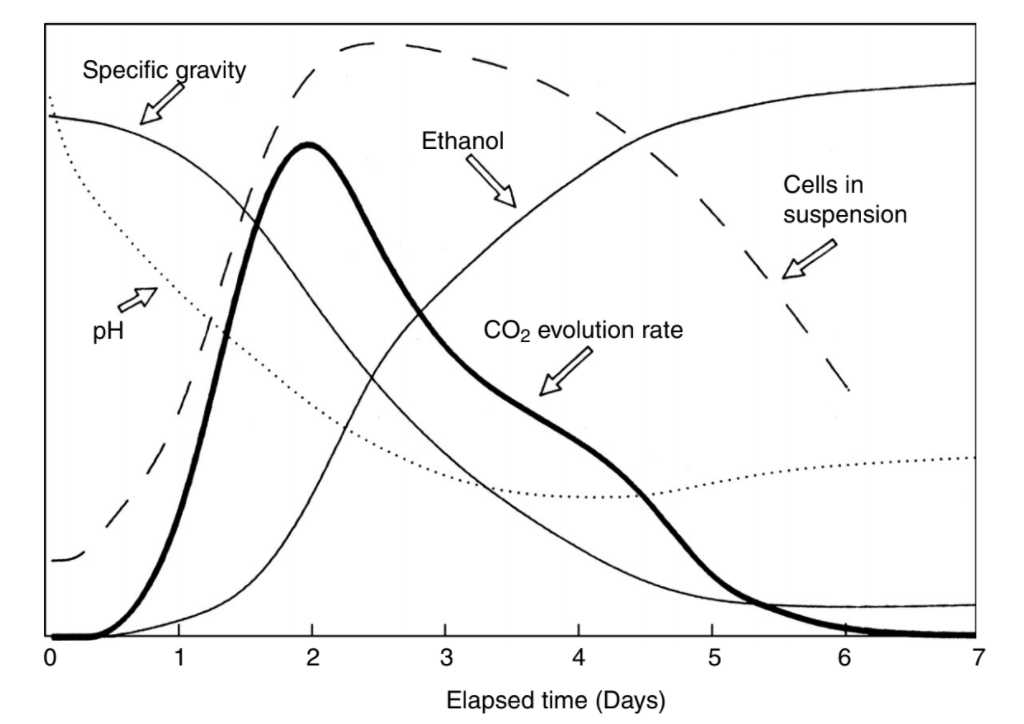
\includegraphics[scale=0.50]{figuras/contexto/variaveis_fermentacao.PNG}
    \caption{Gráfico de evolução de variáveis ao longo da fermentação - Munroe \cite{FermentationMunroe} }
    \label{fig:variaveis_fermentacao}
\end{figure}

\section{Estado da Arte de Sistemas de Produção Artesanal}

\subsection{Análise de Soluções Existentes}

